\documentclass[12pt]{ctexart}
    %%% Document Settings %%%%
%\usepackage[utf8]{inputenc}

\usepackage[
    twoside,
    top=1in,
    bottom=0.75in,
    inner=0.5in,
    outer=0.5in,
]{geometry}
\pagestyle{myheadings}
\usepackage{minted}
\usepackage[dvipsnames,svgnames]{xcolor}

%%%% Additional Commands to Load %%%%
\usepackage{tcolorbox}
\tcbuselibrary{skins}
\tcbuselibrary{minted}
\usemintedstyle{lovelace}
%\usepackage{minted}
\usepackage{color}
\usepackage{tikz}
\usetikzlibrary{calc}
\usepackage{tabularx,colortbl}
\usepackage{amsfonts,amsmath,amssymb}
\usepackage{titling}
\usepackage{mathrsfs}
\usepackage{calc}
\usepackage{subcaption}

\usepackage{listings}
%\usepackage{newtxtext}
\usepackage[strict]{changepage} 
\usepackage{framed}
\definecolor{formalshade}{rgb}{0.95,0.95,1}
\usepackage{float}

%%%% Commands to Define Homework Boxes %%%%
%%%% Box Definition %%%%
\newtcolorbox{prob}[1]{
% Set box style
    sidebyside,
    sidebyside align=top,
% Dimensions and layout
    width=\textwidth,
    toptitle=2.5pt,
    bottomtitle=2.5pt,
    righthand width=0.20\textwidth,
% Coloring
    colbacktitle=gray!30,
    coltitle=black,
    colback=white,
    colframe=black,
% Title formatting
    title={
        #1 \hfill Grade:\phantom{WWWW}
    },
    fonttitle=\large\bfseries
}

%%%% Environment Definition %%%%
\newenvironment{problem}[1]{
    \begin{prob}{#1}
}
{
    \tcblower
    \centering
    \textit{\scriptsize\bfseries Faculty Comments}
    \vspace{\baselineskip}
    \end{prob}
}

\newenvironment{formal}{%
\def\FrameCommand{%
\hspace{1pt}%
{\color{DarkBlue}\vrule width 2pt}%
{\color{formalshade}\vrule width 4pt}%
\colorbox{formalshade}%
}%
\MakeFramed{\advance\hsize-\width\FrameRestore}%
\noindent\hspace{-4.55pt}% disable indenting first paragraph
\begin{adjustwidth}{}{7pt}%
\vspace{2pt}\vspace{2pt}%
}
{%
\vspace{2pt}\end{adjustwidth}\endMakeFramed%
}

    \title{特殊方程作业11}
    \author{地物2201班\ 杨曜堃}
    \date{\today}
%%% document
\begin{document}

% Format Running Header
    \markboth{\theauthor}{\thetitle}
    \maketitle
    \begin{description}
        \item[问题1] 采用拉普拉斯变换法求解下列定解问题$$
        \begin{cases}
            \dfrac{\partial^2u}{\partial t^2}=4\dfrac{\partial^2u}{\partial x^2},&\ 0<x<1,\ t>0\\
            u|_{x=0}=0,\ u|_{x=1}=0,&\ t\geqslant0\\
            u|_{t=0}=0,\ \left.\dfrac{\partial u}{\partial t}\right|_{t=0}=\sin2\pi x,&\ 0\leqslant x\leqslant1
        \end{cases}
        $$
        \item[问题2] 采用积分变换法求解下列定解问题$$
        \begin{cases}
            \dfrac{\partial u}{\partial t}=\dfrac{\partial^2u}{\partial x^2},&\ 0<x<1,\ t>0\\
            u|_{x=0}=100,\ u|_{x=1}=100,&\ t\geqslant0\\
            u|_{t=0}=3\sin(5\pi x)+100,&\ 0\leqslant x\leqslant1
        \end{cases}
        $$
        \item[问题3] 采用适当方法求解下列定解问题$$
        \begin{cases}
            \dfrac{\partial^2u}{\partial x\partial y}=1,&\qquad x>0,\ y>0\\
            u|_{x=0}=y,&\qquad x\geqslant 0\\
            u|_{y=0}=x,&\qquad y\geqslant 0
        \end{cases}
        $$
    \end{description}
    \begin{problem}{问题\#1}
        根据初始条件,确定对$u(x,t)$做关于$t$的拉普拉斯变换,定义
        $$
        U(x,s)\triangleq\int^{\infty}_0u(x,t)e^{-st}\mathrm{d}t
        $$
        由拉普拉斯变换的微分性质
        $$
        \mathscr{L}\left\{\dfrac{\partial u}{\partial t}\right\}=sU(x,s)+u(x,0)=sU(x,s)
        $$
    \end{problem}
    \begin{problem}{问题\#1}
        $$
        \mathscr{L}\left\{\dfrac{\partial^2u}{\partial t^2}\right\}=s^2U(x,s)+u'(x,0)=s^2U(x,s)+\sin2\pi x
        $$
        另一方面
        $$
        \mathscr{L}\left\{\dfrac{\partial^2u}{\partial x^2}\right\}=\dfrac{\mathrm{d}^2U(x,s)}{\mathrm{d}x^2}
        $$
        代入偏微分方程
        $$
        \dfrac{\mathrm{d}^2U(x,s)}{\mathrm{d}x^2}-\dfrac{s^2}{4}U(x,s)=\dfrac{1}{4}\sin2\pi x
        $$
        对应的齐次方程为
        $$
        \dfrac{\mathrm{d}^2U(x,s)}{\mathrm{d}x^2}-\dfrac{s^2}{4}U(x,s)=0
        $$
        解之得齐次方程通解
        $$
        \widetilde{U}(x,s)=C_1e^{-\frac{s}{2}x}+C_2e^{\frac{s}{2}x}
        $$
        观察得到非齐次方程的一个特解
        $$
        U^\ast(x,s)=-\dfrac{\sin2\pi x}{s^2+16\pi^2}
        $$
        从而可以得出非齐次方程的通解
        $$
        U(x,s)=C_1e^{-\frac{s}{2}x}+C_2e^{\frac{s}{2}x}-\dfrac{\sin2\pi x}{s^2+16\pi^2}
        $$
        代入边界条件$U(0,s)=0$,$U(1,s)=0$,得到齐次方程组
        $$
        \begin{cases}
            C_1+C_2=0\\
            C_1e^{-\frac{s}{2}}+C_2e^{\frac{s}{2}}=0
        \end{cases}
        $$
        由于$$
        \left|
        \begin{array}{cc}
            1 & 1 \\
            e^{-\frac{s}{2}} & 2e^{\frac{s}{2}}
        \end{array}
        \right|\neq0
        $$
        说明该齐次方程组只有零解,即$C_1=0$,$C_2=0$
        因此可得
        $$
        U(x,s)=-\dfrac{\sin2\pi x}{s^2+16\pi^2}
        $$
        相应的可以写出拉普拉斯逆变换
    \end{problem}
    \begin{problem}{问题\#1}
        $$
        \mathscr{L}^{-1}\left\{U(x,s)\right\}=-\dfrac{1}{4\pi}\sin2\pi x\sin4\pi t
        $$
    \end{problem}
    \begin{problem}{问题\#2}
        设$u(x,t)=w(x,t)+100$,将定解问题转换成
        $$
        \begin{cases}
            \dfrac{\partial w}{\partial t}=\dfrac{\partial^2w}{\partial  x^2},&\ 0<x<1,\ t>0\\
            w(0,t)=w(1,t)=0,&\ t\geqslant0\\
            w(s,0)=4\sin(5\pi x)
        \end{cases}
        $$
        定义
        $$
        W(x,s)\triangleq\mathscr{L}\{w(x,t)\}=\int^{+\infty}_0w(x,t)e^{-st}\mathrm{d}t
        $$
        $$
        \mathscr{L}\left\{\dfrac{\partial w}{\partial t}\right\}=sW(x,s)+w(x,0)=sW(x,s)+3\sin(5\pi x)
        $$
        $$
        \mathscr{L}\left\{\dfrac{\partial^2w}{\partial x^2}\right\}=\dfrac{\mathrm{d}^2w}{\mathrm{d}x^2}
        $$
        代入偏微分方程,得到常微分方程
        $$
        \dfrac{\mathrm{d}^2w}{\mathrm{d}x^2}-sW(x,s)=3\sin(5\pi x)
        $$
        分别解得齐次方程通解
        $$
        \widetilde{W}(x,s)=C_1e^{-\sqrt{s}x}+C_2e^{\sqrt{s}x}
        $$
        以及非齐次方程特解
        $$
        W^\ast(x,s)=\dfrac{3}{s+25\pi^2}\sin(5\pi x)
        $$
        得到非齐次方程通解
        $$
        W(x,s)=C_1e^{-\sqrt{s}x}+C_2e^{\sqrt{s}x}+\dfrac{3}{s+25\pi^2}\sin(5\pi x)
        $$
        代入边界条件
        $$
        w(0,t)=w(1,t)=0\stackrel{\mathscr{L}}{\longrightarrow}W(0,s)=W(1,s)=0
        $$
    \end{problem}
    \begin{problem}{问题\#2}
        得到齐次方程组
        $$
        \begin{cases}
            C_1+C_2=0\\
            C_1e^{-\sqrt{s}}+C_2e^{\sqrt{s}}=0
        \end{cases}
        $$
        由于
        $$
        \left|
            \begin{array}{cc}
                1 & 1\\
                e^{-\sqrt{s}} & e^{\sqrt{s}}
            \end{array}
        \right|\neq0 
        $$
        所以仅存在零解
        $$
        W(x,s)=\dfrac{3}{s+25\pi^2}\sin(5\pi x)
        $$
        做拉普拉斯逆变换
        $$
        w(x,t)=e^{-(5\pi)^2}\sin(5\pi x)
        $$
    \end{problem}
    \begin{problem}{问题\#3}
        由于
        $$
        \dfrac{\partial^2u}{\partial x\partial y}=1
        $$
        可以设
        $$
        u(x,y)=F(x)+G(y)+xy
        $$
        代入边界条件
        $$
        u(0,y)=F(0)+G(y)=y
        $$
        $$
        u(x,0)=F(x)+G(0)=x
        $$
        整理得
        $$
        F(x)=x-G(0),\ F(0)=-G(0)
        $$
        $$
        G(x)=y-F(0),\ G(0)=-F(0)
        $$
        相应的
        $$
        F(x)=x+F(0)
        $$
        $$
        G(y)=y+G(0)
        $$
        代回原式
        $$
        u(x,y)=xy+x+y+F(0)+G(0)
        $$
    \end{problem}
    \begin{problem}{问题\#3}
        由于$F(0)+G(0)=0$,因此
        $$
        u(x,y)=xy+x+y
        $$
    \end{problem}
    三个问题的结果图示以及MATLAB计算程序附在后面。
    % \begin{lstlisting}[language = Matlab,title={test4\_script.m},  numbers=left, 
    %     numberstyle=\tiny,keywordstyle=\color{blue!70},
    %     commentstyle=\color{red!50!green!50!blue!50},frame=shadowbox,
    %     rulesepcolor=\color{red!20!green!20!blue!20},basicstyle=\ttfamily]
    % \end{lstlisting}
    \begin{figure*}[htbp]
        \small
        \centering
        \subfloat[\label{Fig:a}]{
            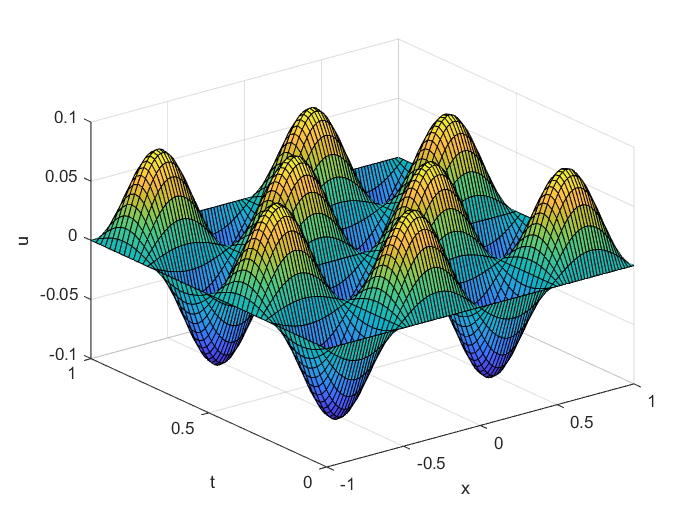
\includegraphics[width=6cm]{fig1.png}
        }
        \subfloat[\label{Fig:a}]{
            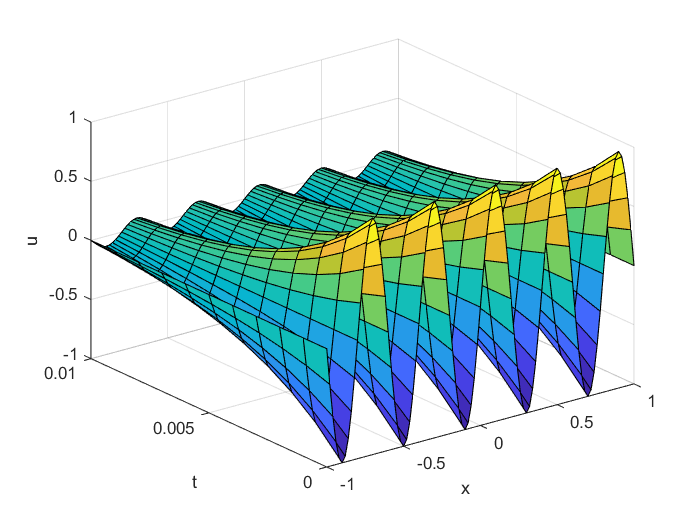
\includegraphics[width=6cm]{fig2.png}
        }
        \subfloat[\label{Fig:a}]{
            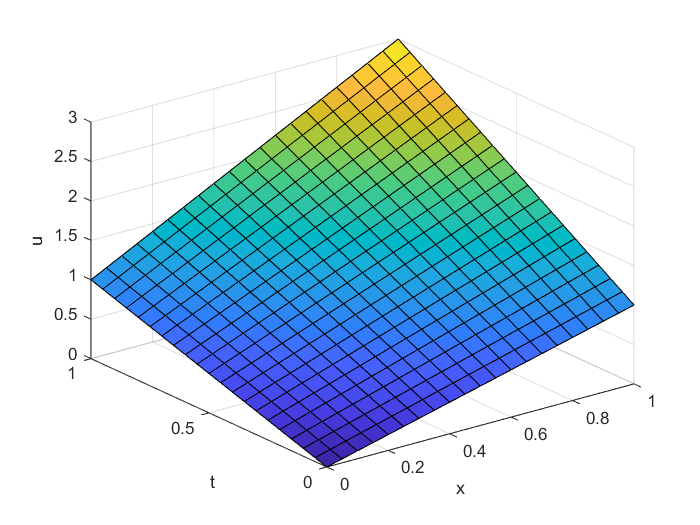
\includegraphics[width=6cm]{fig3.png}
        }
    \end{figure*}
    \begin{figure*}[htbp]
        \small
        \centering
        \subfloat[\label{Fig:a}]{
            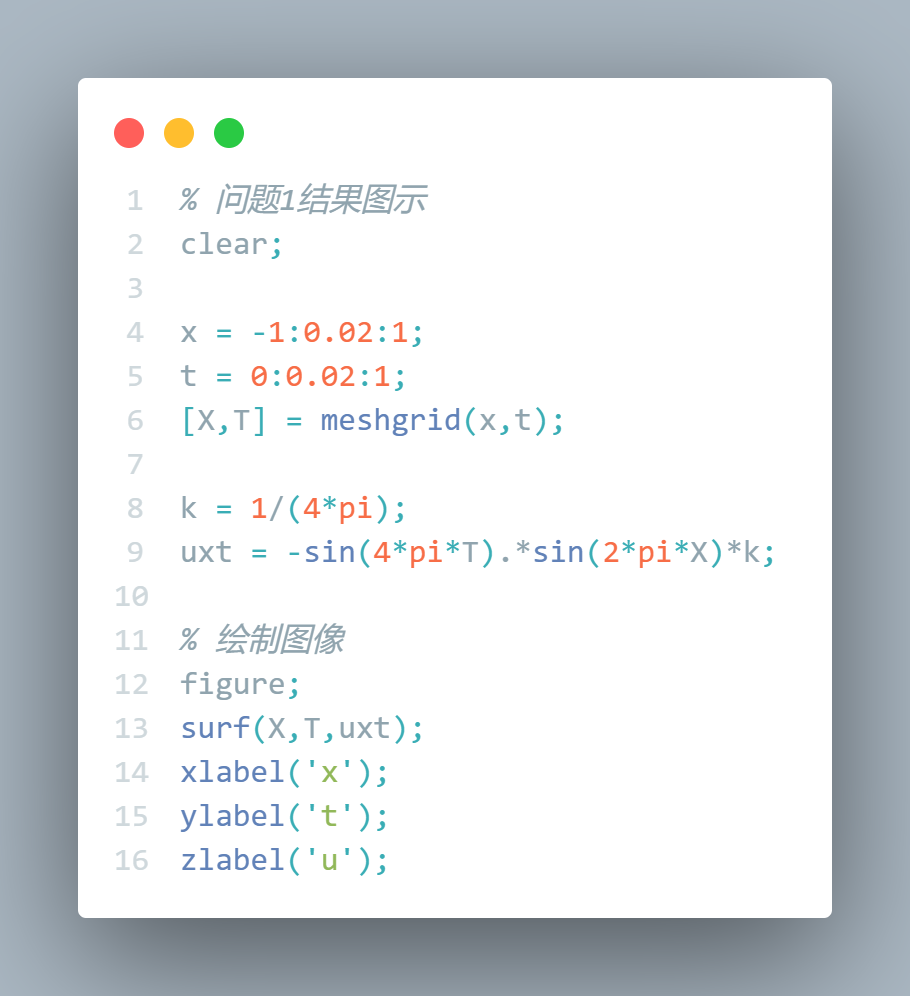
\includegraphics[width=6cm]{code1.png}
        }
        \subfloat[\label{Fig:a}]{
            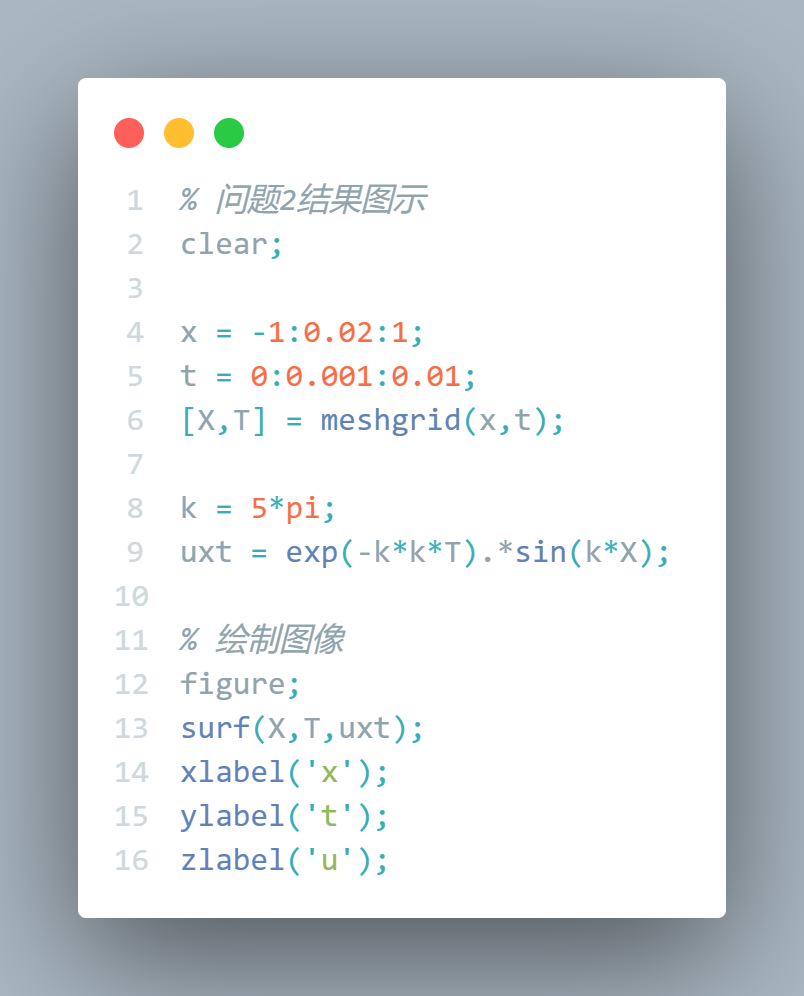
\includegraphics[width=6cm]{code2.png}
        }
        \subfloat[\label{Fig:a}]{
            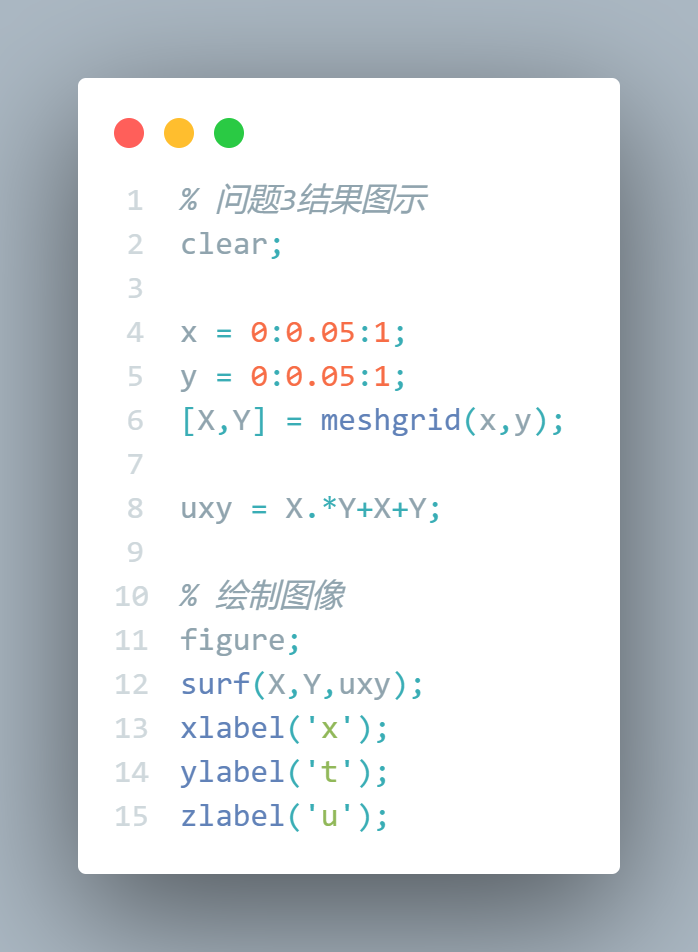
\includegraphics[width=6cm]{code3.png}
        }
    \end{figure*}
\end{document}